\documentclass{standalone}
\usepackage{tikz}
\usetikzlibrary{positioning}

\tikzset{
    no edge from this parent/.style={
        every child/.append style={
        edge from parent/.style={draw=none}}},
    level 4/.style={level distance=6mm}
}

\begin{document}
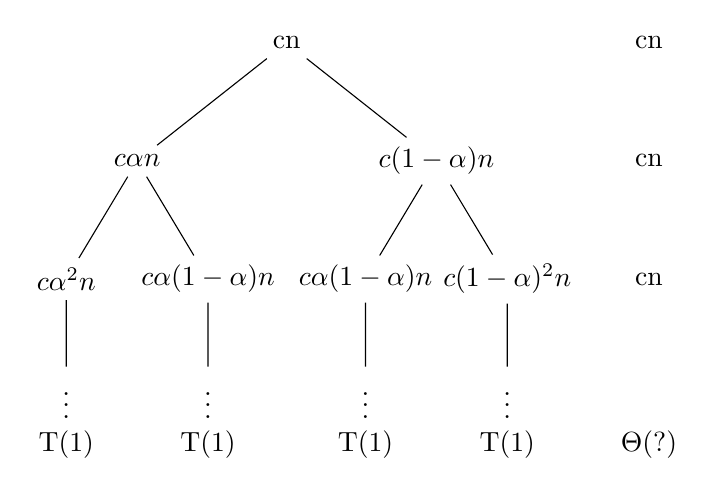
\begin{tikzpicture}
\tikzstyle{level 1}=[sibling distance=38mm]
\tikzstyle{level 2}=[sibling distance=18mm]
\tikzstyle{level 3}=[sibling distance=4mm]

\node (root){cn}
    child {node {$c\alpha{n}$}
        child {node {$c\alpha^2{n}$}
            child {node {$\vdots$}[no edge from this parent]
                child {node {T(1)}}}}
        child {node {$c\alpha(1 - \alpha)n$}
            child {node {$\vdots$}[no edge from this parent]
                child {node {T(1)}}}}}
    child {node {$c(1 - \alpha)n$}
        child {node {$c\alpha(1 - \alpha)n$}
            child {node {$\vdots$}[no edge from this parent]
                child {node {T(1)}}}}
        child {node {$c(1 - \alpha)^2n$}
            child {node {$\vdots$}[no edge from this parent]
                child {node {T(1)}}}}};

\node[right=4 of root] {cn}[no edge from this parent]
    child {node {cn}[no edge from this parent]
        child {node {cn}[no edge from this parent]
            child {node {}[no edge from this parent]
                child {node {$\Theta(?)$}}}}};
\end{tikzpicture}
\end{document}